\pgfplotsset{width=0.72\linewidth,height=3.2cm,compat=1.18}
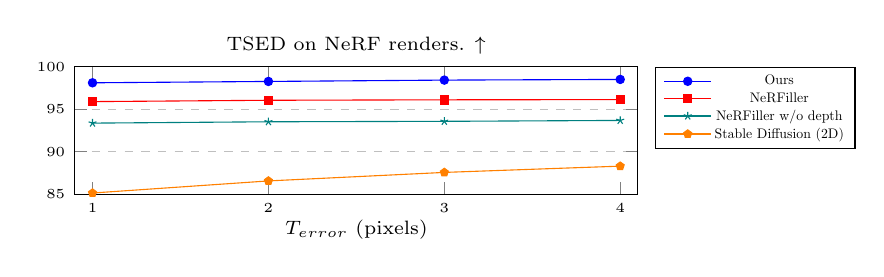
\begin{tikzpicture}
    \begin{axis}[
        title style={align=center, font=\scriptsize, yshift=-.5em},
        title={TSED on NeRF renders. $\uparrow$},
        xlabel={$T_\text{error}$ (pixels)},
        xmin=0.9, xmax=4.1,
        ymin=85, ymax=100,
        xtick={1,2,3,4},
        ytick={85,90,95,100},
        legend pos=outer north east,
        legend style={nodes={scale=0.5, transform shape}},
        label style={font=\scriptsize},
        tick label style={font=\tiny},
        ymajorgrids=true,
        grid style=dashed,
        xlabel style={yshift=1ex},
        ylabel style={yshift=-1.5ex},
        mark size=1.5pt,x
    ]
        \addplot[color=blue,mark=*,] coordinates {
        (1.0,98.1013)(2.0,98.2595)(3.0,98.4177)(4.0,98.4968)
        };
        \addplot[color=red,mark=square*,] coordinates {
        (1.0,95.8861)(2.0,96.0443)(3.0,96.0970)(4.0,96.1234)
        };
        \addplot[color=teal,mark=star,] coordinates {
        (1.0,93.3544)(2.0,93.5127)(3.0,93.5654)(4.0,93.6709)
        }; 
        \addplot[color=orange,mark=pentagon*,] coordinates {
        (1.0,85.1266)(2.0,86.5506)(3.0,87.5527)(4.0,88.2911)
        }; 
        \legend{Ours ,NeRFiller ,NeRFiller w/o depth, Stable Diffusion (2D)}
    \end{axis}
\end{tikzpicture}
